%!TEX root = geometry.tex
\stepcounter{lecture}
\setcounter{lecture}{7}
\sektion{Surfaces}

\subsection{First fundamental form} % (fold)
\label{sub:first_fundamental_form}

Suppose $\sigma:U \to \R^3$ is a parameterised surface $S$ and let $g$ be the induced metric on $U$.

\begin{definition}
	The \emph{first fundamental form} at a point $p\in U$ is the bilinear form on $\R^2$ given by
	\begin{equation*}
		B_{I,p} := g_p(\vv,\ww).
	\end{equation*}
	This is represented by the matrix
	\begin{equation*}
		\mat{\sigma_x \\ \sigma_y} \mat{\sigma_x & \sigma_y} = \mat{\bsig_x \cdot \bsig_x & \bsig_x \cdot \bsig_y \\ \bsig_y \cdot \bsig_x & \bsig_y \cdot \bsig_y} = \mat{E & F \\ F & G}.
	\end{equation*}
\end{definition}

% subsection first_fundamental_form (end)

\subsection{Second fundamental form} % (fold)
\label{sub:second_fundamental_form}

The tangent space $T_{\sigma(p)} S$ is spanned by $\dif{\sigma_p}(1,0) = \bsig_x$ and $\dif{\sigma_p}(0,1) = \bsig_y$.

The unit normal to $T_{\sigma(p)} S$ at $\sigma(p)$ is
\begin{equation*}
	\nn(p) = \f{\bsig_x \cross \bsig_y}{\left\vert \bsig_x \cross \bsig_y \right\vert}.
\end{equation*}
The map $\nn:U\to S^2 \subset \R^3$ is called the \emph{Gauss map}.

\begin{definition}
	The \emph{second fundamental form} of $\sigma$ at $\pp$ is the bilinear form on $\R^2$ defined by
	\begin{equation*}
		B_{\text{\emph{II}},p}(\vv,\ww) = -\dif{\sigma_p(\vv)} \cdot \dif{\nn_p}(\ww)
	\end{equation*}
\end{definition}

There's a useful procedure for computing it. Let
\begin{itemize}
	\shortskip
	\item $S=\mat{\sigma_x & \sigma_y}$ be the $3\times 2$ matrix that represents $\dif{\sigma}$; and
	\item $N=\mat{\nn_x & \nn_y}$ be the matrix that represents $\dif{\nn}$.
\end{itemize}
Then we have
\begin{equation*}
	B_{\text{\emph{II}}}(\vv,\ww) = -(S\vv)^\Trans (N\ww)
	= - v^\Trans S^\Trans N \ww
	= -\vv^\Trans \mat{\sigma_x \\ \sigma_y} \mat{\nn_x & \nn_y} \ww.
\end{equation*}
Thus $B_{\text{\emph{II}}}$ is given by the matrix
\begin{equation*}
	-\mat{\sigma_x \\ \sigma_y} \mat{n_x & n_y}
	= -\mat{\sigma_x \cdot n_x & \sigma_x \cdot \nn_y \\ \sigma_y \cdot n_x & \sigma_y \cdot n_y}
	= \mat{L & M_1 \\ M_2 & N}.
\end{equation*}

\begin{lemma}
	\begin{equation*}
		\mat{L & M_1 \\ M_2 & N} = \mat{\sigma_{xx} \cdot \nn & \sigma_{xy} \cdot \nn \\ \sigma_{yx} \cdot \nn & \sigma_{yy} \cdot \nn}
	\end{equation*}
\end{lemma}

\begin{proof}
	If $\sigma_x \in T_{\sigma(p)} S$, then $\sigma_x \cdot \nn = 0$. Then $\sigma_{xx} \cdot \nn + \sigma_x \cdot \nn_x = 0$, so $-\sigma_x \cdot n_x = \sigma_{xx} \cdot \nn$. Thus $L=\sigma_{xx} \cdot \nn$. Other entries are similar.
\end{proof}

\begin{corollary}
	$B_{\text{\emph{II}}}$ is symmetric.
\end{corollary}

\begin{proof}
	We have $\sigma_{xy} = \sigma_{yx}$, so done.
\end{proof}

	\pagebreak

\begin{example}
	We have $\sigma(\theta,z) = (\cos \theta, \sin\theta, z)$; a cylinder of radius $1$. Thus
	\begin{equation*}
		\sigma_\theta=(-\sin \theta, \cos\theta, 0) \qqand
		\sigma_z= (0,0,1).
	\end{equation*}
	Then we have
	\begin{equation*}
		\mat{E & F \\ F & G} = \mat{1 & 0 \\ 0 & 1} \qqand
		g =\dif{z^2} + \dif{\theta^2},
	\end{equation*}
	so this is locally Euclidean. Thus the normal is
	\begin{equation*}
		\nn
		= \f{\sigma_\theta \cross \sigma_z}{\left\vert \sigma_{\theta} \cross \sigma_z \right\vert}
		= (\cos\theta, \sin\theta, 0)
	\end{equation*}
	Taking second derivatives gives
	\begin{equation*}
		\sigma_{\theta\theta} = (-\cos\theta, -\sin\theta,0) \qqand
		\sigma_{\theta z} = \sigma_{zz} = 0.
	\end{equation*}
	Thus our matrix is given by
	\begin{equation*}
		\mat{L & M \\ M & N} = \mat{-1 & 0 \\ 0 & 0} \qqand
		B_{\text{\emph{II}}} = \dif{\theta^2}.
	\end{equation*}
\end{example}

\begin{theorem}
	[Gauss' theorema egregium] If $g$ is the metric induced by $\sigma$, then
	\begin{equation*}
		K_p(g)
		= \f{\det(B_{\text{\emph{II}}}(\sigma))}{\det(B_I(\sigma))}
		= \f{LN-M^2}{EG-F^2}.
	\end{equation*}
\end{theorem}

\emph{See handout.}

% subsection second_fundamental_form (end)

% This was labelled section 7.4, but it's only 7.3 in LaTeX. Am I missing something?

\subsection{Closed surfaces and charts} % (fold)
\label{sub:closed_surfaces_and_charts}

We have the following basic problem:
\lecturemarker{16}{13 Mar}

\textbf{Problem.} A compact surface $S$ (such as the sphere $S^{\,2}$) cannot be written as the image of a single map $\sigma: U\to S$, where $U$ is open in $\R^2$.

This is actually a theorem, which can be proved using \emph{Algebraic Topology}.

\emph{Solution.} Cover $S$ with open sets, each of which is parameterised. This gives us something close to what we want. We require the following definition:

\begin{definition}
	If $S \subset \R^3$, a \emph{chart} for $S$ is an open set $V \subset S$ and a bijective map $f:V \xrightarrow{\text{open}} \R^2$ such that $\sigma = f^{-1}$ is a parametrisation.

	It might seem strange to think of the inverse of the map, but later it will be more convenient to think of charts in this way.

	If $f_i:V_i \to U_i$, $i=1,2$ are two charts on $S$, then the \emph{transition function} $\phi_{12}: f_1(V_1 \cap V_2) \to f_2 (V_1 \cap V_2)$ is given by $\phi_{12} = f_2 \circ f_1^{-1}$.

	We say that $f_1$ and $f_2$ are \emph{compatible} if $\phi_{12}$ and $\phi_{21} = \phi_{12}^{-1}$ are both differentiable.
	% \missingfigure{Geo 16/1}
\end{definition}

This might seem like a strange statement to make, because after some algebra we can prove that it always holds for embedded surfaces (the only surfaces that we've been considering). But later, when we consider abstract surfaces, this will turn out to be very useful.

\begin{definition}
	An \emph{atlas} for $S\subset \R^3$ is a set of compatible charts $f_i: V_i \to U_i$ such that the $V_i$ covers $S$. We say $S$ is an \emph{embedded surface} in $\R^3$ if it has an atlas.
\end{definition}

\begin{example}
	An atlas for $S^{\,2} \subset \R^3$ is
	\begin{itemize}
		\shortskip
		\item $\pi_1:S^2-\{N\} \to \R^2$ is stereographic projection from the north pole $N$;
		\item $\pi_2:S^2-\{S\} \to \R^2$ is stereographic projection from the north pole $S$.
	\end{itemize}
	We treat $\R^2-\{0\}$ as $\C^*$, and then our transition function is
	\begin{equation*}
		\fullfunction{\phi_{12}}{\C^*}{\C^*}{z}{1/\overline{z}}.
	\end{equation*}
\end{example}

\subsubsection*{Metrics} % (fold)
\label{ssub:metrics}

If $f_1,f_2$ are compatible charts on $S$, then $f_i^{-1}$ induces a Riemannian metric $g_i$ on $U_i$,, given by
\begin{equation*}
	g_i(\vv,\ww) = (\dif{f_i})^{-1}(\vv) \cdot (\dif{f_i^{-1}})(\ww).
\end{equation*}

\begin{lemma}
	$\phi_{12}:(f_1(V_1 \cap V_2), g_1)) \to (f_2(V_1 \cap V_2), g_2)$ is an isometry.
\end{lemma}

\begin{proof}
	Working through the algebra:
	\begin{align*}
		g_2(\dif{\phi_{12}(\vv)}, \dif{\phi_{12}(\ww)})
		&= (\dif{f_2})^{-1} (\dif{f_2} \circ (\dif{f_1})^{-1} (\vv)) \cdot \dif{f_2^{-1}}(\dif{f_2} \cdot (\dif{f_1})^{-1}(\ww)) \\
		&= \dif{f_1^{-1}}(\vv) \cdot \dif{f_1^{-1}}(\ww) \\
		&= g_1(\vv,\ww). \qedhere
	\end{align*}
\end{proof}

If $S\subset \R^3$ is a smoothly embedded surface, and $p\in S$, then the Gauss curvature is given by $K_p(S) := K_{f(p)}(g)$, where $f:V\to U$ is a chart defined in a neighbourhood of $p$ and $g$ is the metric induced on $f$.

The lemma implies that this is well-defined.

Similarly, $\gamma:(a,b) \to S$ is a geodesic if $f\circ \gamma$ is a geodesic with respect to the metric $g$ induced by $f$, where $f$ is any chart of $S$.

% subsubsection metrics (end)

% subsection closed_surfaces_and_charts (end)

\subsection{Abstract surfaces} % (fold)
\label{sub:abstract_surfaces}

Suppose $S$ is a Hausdorff, second-countable topological space. A chart on $S$ is an open set $V\subset S$ and a bijective map $f:V\to U \subset \R^2$, with $U$ open. (Don't worry if some of these terms are unfamiliar; they will be introduced formally in \emph{Metric \& Topological Spaces}. They are cited here merely for completeness.) Many definitions are the same as with closed surfaces:

If $f_1,f_2$ are charts on $S$, then the transition function $\phi_{12}:f_1(V_1 \cap V_2) \to f_2(V_1 \cap V_2)$ is given by $\phi_{12} = f_2 \circ f_1^{-1}$.

We say that $f_1$ and $f_2$ are compatible if $\phi_{12}$ are differentiable. This definition is exactly the same as before, but now it has teeth. In the embedded case, we merely need to ask that $f_1^{-1}$ be differentiable for $f_1$ and $f_2$ to be compatible. In this case, it doesn't make sense to ask that $f_1^{-1}$ be differentiable, so this is actually a useful distinction to make.

An atlas on $S$ is a set of compatible charts $f_i:V_i \to U_i$ such that the $V_i$ cover all of $S$.

\begin{definition}
	An \emph{abstract smooth surface} is a space $S$ as above together with an atlas on $S$.
\end{definition}

In some sense, there's nothing special about two dimensions in this definition. We could similarly define an abstract smooth $n$-manifold. Some other properties aren't so nice though. There are some four-manifolds which don't admit any structure as a smooth manifold, whereas $\R^4$ can be made into a smooth manifold in uncountably many ways.

In almost all cases, it is better to think about smooth manifolds, but these are not discussed in this course. We mention them here only for completeness, and will henceforth restrict our discussion to surfaces.

\begin{example}
	Consider the torus $T^2=\R^2/\Z^2$. There is a projection map $\pi:\R^2\to T^2$.
	Charts on $T^2$ are inverses of maps $\pi_U:U \to T^2$, the restriction of $\pi$ to an open set $U=B_\epsilon(p)$, $\epsilon<1/2$.
	% 
	% ensure that ball does not overlap itself when projected
	% inverse of map gives a triangle
	%
	Transition functions are translations by $(n,m)\iZ^2$.
\end{example}

\begin{definition}
	If $\left\{f_i:V_i \to U_i\right\}$ is an atlas on an abstract surface $S$, then a Riemannian metric on $S$ is a set of metrics $g_i$ on $U_i$ so that the transition functions $\phi_{ij}(f_i(V_i \cap V_j), g_i) \to (f_j(V_i \cap V_j), g_j)$ are all isometries.
\end{definition}

In an embedded surfaces, we get these as isometries for free. Here, we have to include it as part of the definition.

\begin{example}
	The flat metric on $T^2$ is defined by taking the atlas in the previous example, and equipping each $U$ with the Euclidean metric $\dif{x^2} + \dif{y^2}$. The transition functions are all translations, so isometries under $g^E$. The Gauss curvature of $g$ is identically zero.

	However, there is no way to embed $T^2$ into $\R^3$ such that the Gauss curvature is identically zero (see examples sheet).

	In some sense, it is better to think of this embedding as treating $T^2$ as the quotient of $(\R^2, g^E)$, by the action of a group of isometries.
\end{example}

Here the phrase \emph{flat metric} is used to describe a surface (or manifold) with identically zero Gauss curvature.

\begin{example}
	The Möbius strip also has a flat metric. The strip is given by $M=\R\times (-1,1)/G$, where $G\cong \Z$ and $K\cdot(X,Y) = (x+k, \left( -1 \right)^k + y)$. (Take the two sides of an infinite strip and glue them together with a strip, as we illustrated previously.) Again, this is an isometry of the Euclidean metric.
\end{example}

% subsection abstract_surfaces (end)

	\pagebreak

\subsection{Global Gauss-Bonnet} % (fold)
\label{sub:global_gauss_bonnet}

This leads us to the final theorem of the course, generalising the local Gauss-Bonnet theorem we saw previously:

\begin{theorem}
	If $(S,g)$ is a compact abstract surface equipped with a Riemannian metric $g$, then
	\begin{equation*}
		2\pi \,\chi(S) = \int_S K(g) \dif{A_g}.
	\end{equation*}
\end{theorem}

There are all sorts of beautiful theorems like this, which relate global topological information to local properties. This is not an isolated example, although it is the only such theorem we study in this course.

\begin{example}
	Take $S=S^{\,2}$ and let $g=g^{\,S}$ be the spherical metric. We know Gaussian curvature is $K \equiv 1$. Then
	\begin{equation*}
		2\pi \cdot 2 = \int_{S^2} 1 \dif{A} = 4\pi,
	\end{equation*}
	and everything is consistent.
\end{example}

The idea behind the theorem is quite easy. Technical details are needed to make it into a complete proof; here we present the main ideas.

\begin{proof}
	[Sketch proof] Find a geodesic triangulation of $S$ (that is, a triangulation where edges are geodesics), and so that each face is contained in a chart.
	% 
	The idea is to start with any triangulation, and subdivide the edges, replacing small edges by geodesics.
	
	\begin{center}
		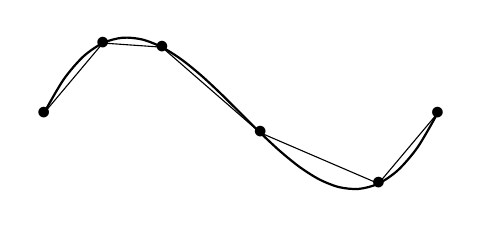
\begin{tikzpicture}[scale=2.5]
			\draw [thick] plot [smooth] coordinates {(-1,0) (-0.9, 0.171) (-0.8, 0.288) (-0.7, 0.357) (-0.6, 0.384) (-0.5, 0.375) (-0.4, 0.336) (-0.3, 0.273) (-0.2, 0.192) (-0.1, 0.099) (0,0) (0.1, -0.099) (0.2, -0.192) (0.3, -0.273) (0.4, -0.336) (0.5, -0.375) (0.6, -0.384) (0.7, -0.357) (0.8, -0.288) (0.9, -0.171) (1,0)}; %
			
			\foreach \s/\t/\u/\v in {-1/0/-0.7/0.357, -0.7/0.357/-0.4/0.336, -0.4/0.336/0.1/-0.099, 0.1/-0.099/0.7/-0.357, 0.7/-0.357/1/0}
			{
				\draw (\s,\t) -- (\u,\v);
				\draw (\s,\t) node {$\bullet$};
			}
			
			\draw (1,0) node {$\bullet$};
			
		\end{tikzpicture}
		\end{center}

	Importantly, this does not change the topology of the triangulation.

	Now suppose triangulation has $V$ vertices, $E$ edges and $F$ faces. We know that $E=\f{3}{2}F$ (recall our discussion of the Euler characteristic for the sphere). Then
	\begin{align*}
		\iint_S K \dif{A_g}
		&= \sum_{i=1}^F \iint_{f_i} K \dif{A_g} \\
		\intertext{where $f_i$ is the $i$th face. Then we apply local Gauss-Bonnet, and letting $\alpha_{ij}$, $j=1,2,3$ be the angles in $f_i$:}
		&= \sum_{i=1}^F \defect(f_i) \\
		&= \sum_{i=1}^F \left( \alpha_{i1} + \alpha_{i2} + \alpha_{i3} - \pi \right) \\
		&= \sum_{i,j} \alpha_{ij} - \pi F
		 = 2\pi V - \pi F
		 = 2\pi\left( V-E+F \right). \qedhere
	\end{align*}
\end{proof}

% subsection global_gauss_bonnet (end)
